\chapter{Design and Implementation}
\label{chap:design}
\section{Docker}
Native Docker has two parts, Docker Client and Docker Daemon. Docker Daemon has several components include server, engine, registry, graph, driver and runC. To support Checkpoint and Restoration request, some of these steps should be implemented.

\subsection{Docker Client}
There are 3 Docker commands implementation in Docker Client, including Checkpoint, Restore, and Migrate. In Checkpoint command should have these configurations:
\begin{itemize}
	\item Image directory - Dump checkpoint image directory.
	\item Work directory - Dump checkpoint image log directory.
	\item Leave running - After dumping the checkpoint images, consideration is required whether the container keep running.
	%consideration is required whether the container keep running.
	\item Pre-dump - Pre-dump checkpoint memory image to minimize frozen time.
	\item Pre image directory - Define which version image to compare.
	\item Track memory - Track memory to pre image directory image to minimize disk space.
\end{itemize}
In Restore command, it should have these configurations:
\begin{itemize}
	\item Image directory - Checkpoint image directory to restore from.
	\item Work directory - Directory for restore log.
	\item Force - Force restoring the container from image directory whether container is running.
\end{itemize}
In Migrate command, it focuses on Docker Swarm Scheduler filter configurations. Meanwhile, in Run command, it is possible for the container to set filter configurations with environment variables or labels. Therefore, the implementation of environment variables and labels in Migrate command is required.

\subsection{Docker Daemon}
In native Docker Daemon, it does not support Checkpoint and Restore commands.
Fortunately, it is already implemented in runC, so we have to add a proxy between Docker Daemon and runC, which can handle Docker Client's Checkpoint and Restore requests.

\section{Docker Swarm Configuration}
As Figure \ref{fig:Docker Swarm with remote storage server}, it shows a remote storage server for saving Docker containers dump checkpoint images and it should have fault tolerant to avoid service shutdown.

\begin{figure}[h]
\begin{center}
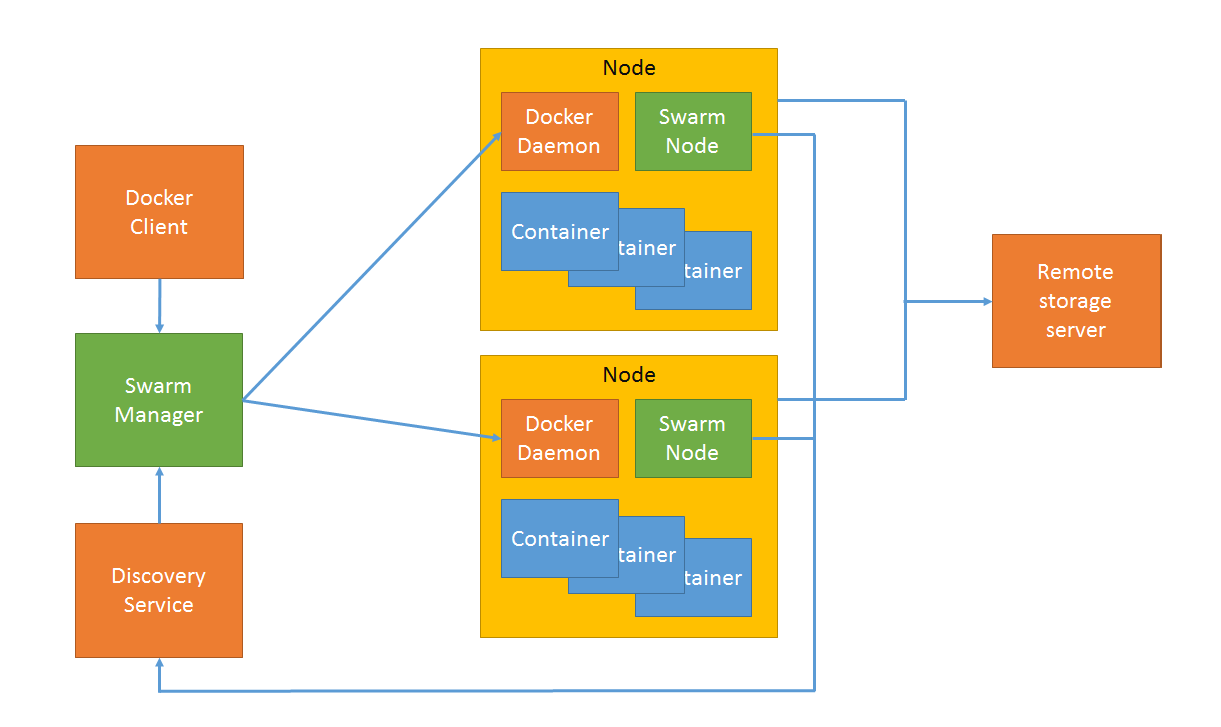
\includegraphics[width=15cm]{figure/swarm_docker_remote.png}
\end{center}
\caption{Docker Swarm with remote storage server}
\label{fig:Docker Swarm with remote storage server}
\end{figure}

\section{Docker Containers Migration in Docker Swarm}
Docker Swarm creates containers through Swarm scheduler to dispatch Docker nodes. If a specific node needs to be assigned to create a container, Swarm schedule parameter should be set.
In migrating a container in Docker Swarm, the Swarm schedule parameter should be assigned in order to avoid the container to restore to the same node.
\begin{enumerate}[Step 1.]
	\item Check Docker Swarm cluster has at least two Swarm nodes.
    \item Parse Docker Client requests to analyse label and environment variables, and transform label and environment variables to Docker Swarm filters.
    \item The Swarm schedule parameter should be added to make sure the container will not be migrated to the same node.
    \item Create empty container on the Docker Swarm scheduler which node its pointing to, this could lead to downloading the container image if it doesn't exist in the be chosen node.
    \item Pre-dump the container's checkpoint images which we want to migrate to decrease container's frozen time.
    \item Dump the container's checkpoint images by tracking memory from the pre-dumped checkpoint images.
    \item Restore the container's checkpoint images to the empty container that Docker Swarm scheduler points to.
    \item Delete the checkpoint images.
    \item If the container has been migrated which has set the Checkpoint and Restoration Rescheduling Policy, it will restart the Checkpoint and Restoration Rescheduling Policy \ref{sec:checkpoint restore rescheduling policy}.
\end{enumerate}
%
%The first step of creating the container in another Swarm Node is quicker for all environments, because we assume that they already have downloaded their container images from the remote repository, thus, they don't need to transport container images from the other Swarm Node.
%
%Second, if we have version control of checkpoint the container, the container has to pre-dump the checkpoint image. After pre-dumping the checkpoint image, 

\section{Docker Swarm Checkpoint and Restoration \\Rescheduling Policy}
\label{sec:checkpoint restore rescheduling policy}
In Docker Swarm, it has Rescheduling Policy. As the reschedule policy is set when we start a container, whenever Swarm nodes fail, Swarm Manager will restart the containers to another alive Swarm Nodes.

To improve this policy, a Checkpoint Ticker should be needed to keep every containers' checkpoints up to date.
Whenever Swarm Nodes fail, Swarm Manager will restore the containers which their checkpoints have been dumped by Swarm Manager to the remote storage server.
Otherwise, the Checkpoint Ticker provides the version of checkpoint image by tracking memory. It only dumps the different memory pages' checkpoint to new version checkpoint images.

By experiment results, when many containers checkpoint in the same time, all of the containers checkpoint time will increase, especially the remote storage is hard disk.
To avoid many containers checkpoint in the same time, the checkpoint requests from different containers will be collected in a checkpoint queue.
It only allows one container checkpoint at a time.

In addition, Docker Swarm Checkpoint and Restoration Rescheduling Policy also supports high availability whenever Docker Swarm primary manager fails, the others Swarm Manager replica instances will lead to a new primary manager. After replica has chosen a new primary manager, it will restart the container's Checkpoint Tickers.
By experiment, it can save at least 2 times storage space when $VG_i$ bigger than 5.

\subsection{Docker Swarm Container Checkpoint Ticker}
Algorithm \ref{code:checkpointTicker} shows the Container Checkpoint Ticker's algorithm.
In line 1 and 2, checkpoint-time period $T_i$ and version-group $VG_i$ are set when the container $C_i$ is created through Docker Swarm Manager, and every $T_i$ is independent.
Each $T_i$ in the Docker Swarm cluster has its starting time and time ticker, time ticker will dump checkpoint image repetitively at regular intervals. If version-group $VG_i$ has not been set, it will be set to 5.
Checkpoint version $V_i=0$ and pre-dump checkpoint version $pre$-$dump V_i=0$ should be defined for each container $C_i$.

In line 4 to 18, for each container is running and $C_i$ checkpoint ticker period $T_i$ pounds, $C_i$, Swarm Manger will do line 5 to 17.
In line 6 to 11, if the container $C_i$ does not has any pre-dump image, newest version-group $VG_i$ checkpoint is full or previous pre-dump average images size over 500 MB, Swarm Manger will send the request to Swarm Node $N_i$ to create a new directory and pre-dump the checkpoint image as pre-dump version $pre$-$dump V_i$.
After pre-dumping the container checkpoint image or $C_i$ has previous version checkpoint images, Swarm Manager will send requests to dump checkpoint image to Swarm Node $N_i$ to dump checkpoint version $V_i$. Whenever dumping checkpoint image, CRIU will track the memory difference to the previous checkpoint images or the pre-dumping checkpoint images to reduce image disk space usage.
As it is shown as Figure \ref{fig:Containers checkpoint versions in remote storage server}, every container has each pre-dump checkpoint directories and each pre-dump checkpoint directories have version-group versions checkpoint images.
In line 12 to 14, Swarm Manager sends delete checkpoint request to $N_i$ to delete oldest Pre-dump version directory whenever container has more than three Pre-dump versions directory.

\begin{figure}[h]
\begin{center}
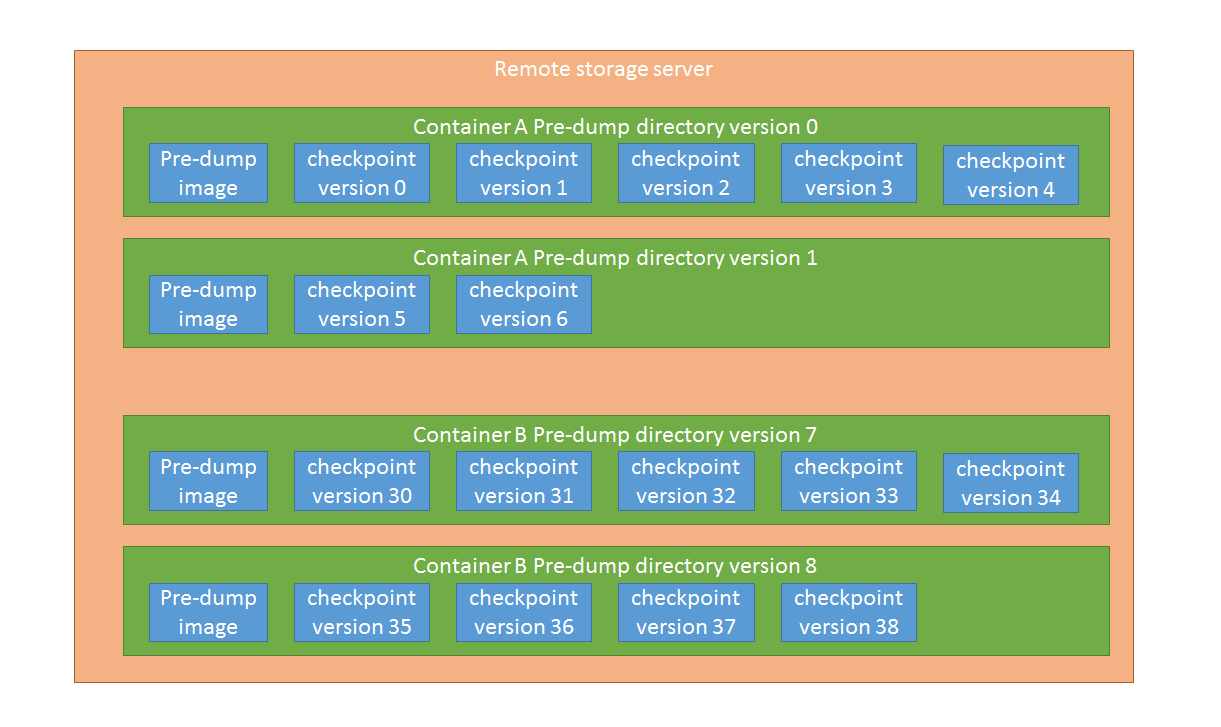
\includegraphics[width=15cm]{figure/checkpoint_demo.png}
\end{center}
\caption{Containers checkpoint versions in remote storage server}
\label{fig:Containers checkpoint versions in remote storage server}
\end{figure}

\begin{algorithm}[h]
    \caption{Checkpoint Ticker Algorithm}
    \label{code:checkpointTicker}
    \begin{algorithmic}[1]
	\Require
		The set of Swarm Nodes: $\lbrace N_1,N_2,...,N_m \rbrace $;
		The set of containers: $\lbrace C_1,C_2,...,C_n \rbrace$;
		Version-group: $ VG_i $;
		Checkpoint-ticker period: $ T_i $;
	\Ensure
		pre-dump images $ pre$-$dump V_i $; dump images $ V_i $ ;
        \State Set $ T_i $ and $ VG_i $ labels when create the container $ C_i $;
        \State initial $ V_i=0 $, $ pre$-$dump V_i=0 $;
        \\
		\For {each $ C_i $ in $ N_i $}
			\While {$ C_i $ running $ \& $ $ T_i $ pounding}
				\If {version $ \% $ $ VG_i $ == 0 }
					\If {$ pre$-$dump V_i - 1$ average images size$ < $  500 MB}
						\State add pre-dump checkpoint image $ pre $-$ dump V_i $ request to queue;
					\EndIf
				\EndIf
			\State add dump checkpoint image $ V_i $ request to queue;
				\If { $ VG_i$ directory $ > $ 3 } 
                	\State delete oldest pre-dump checkpoint $ pre $-$ dump V_i $ directory;
				\EndIf
            	\State $ V_i $ = $ V_ i$ + 1;
            	\If {$ V_i $ $\%$ $VG_i$ == 0 } 
					\State $ pre $-$ dump V_i $ = $ pre $-$ dump V_i $ + 1;
				\EndIf
			\EndWhile
		\EndFor
	\end{algorithmic}
\end{algorithm}

\subsection{Docker Swarm Restore Rescheduling Policy}
Algorithm \ref{code:Restore} gives a specific explanation of Restore Rescheduling Policy. In line 1, $ R_i $ label is set when the container $C_i$ is created by Docker Swarm Manager.
In line 3 to 7, whenever Swarm Nodes $ N_i $ fail, Swarm Manager will execute procedure \textsc{Restore container} that restores every container $ C_i $ which has $ R_i $ label to another Swarm Nodes $ N_i $.

In line 9 to 21, each container $ C_i $ executes procedure \textsc{Restore container}; Swarm Manager will choose a Swarm Node $ N_r $ and create an empty container $ C_r $ in $ N_r $. In this step, Swarm Manager will check whether $ N_r $ has the container's image. If $ N_r $ doesn't have the container's image, $ N_r $ will download the container's image from Docker remote registry and create the empty container $ C_r $.
As result of creating container $ C_r $, Swarm Manager restores the fail container $ C_i $ checkpoint image to $ C_r $. To avoid a fail restoration, Swarm Manager will retry to restore the second last version's checkpoint, and it will retry version-group $ VG_i $ (default is 5) for several instances. The container $ C_i $ checkpoint image will be removed after restoring the container $ C_i $.

Whenever Swarm Manager's attempts to retry are all failed for $ VG_i $ times, it will create and restart a new container as normal Docker Swarm Rescheduling Policy.

\begin{algorithm}[h]
    \caption{Restore Rescheduling Algorithm}
    \label{code:Restore}
    \begin{algorithmic}[1]
    	\Require
		The set of Swarm Nodes: $ \lbrace N_1,N_2,...,N_m \rbrace $;
		The set of containers: $ \lbrace C_1,C_2,...,C_n \rbrace $;
		Version-group: $ VG_i $;
		Checkpoint-ticker period: $ T_i $;
		Restore rescheduling policy label:$ R_i $;
	\Ensure
		Restored containers:$ C_{ri} $;
        \State Set $ R_i $ labels when creating the container;
        \\
        \If {$ N_i $ fail}
        	\ForAll{$ C_i $ in fail $N_i$ has $ R_i $}
        		\State \textsc{Restore Container};
        	\EndFor
        \EndIf
        \\
        \Procedure{Restore Container}{}
			\State $ N_r $ $\longleftarrow$Create a empty container $ C_r $
			\For {$ V_i $ downto $ V_i $ - $ VG_i $}
				\State $ C_{ri} $ $\longleftarrow$ Restore checkpoint $ V_i $;
				\If{ Restore $ C_{ri} $ success }
					\State \textbf{break}
				\EndIf
			\EndFor
			\State Delete the container checkpoint image;
			\If{Restore container $C_i$ fail}
				\State $ C_r \longleftarrow $ Restart the container; $C_i$;
			\EndIf
		\EndProcedure
	\end{algorithmic}
\end{algorithm}

\subsection{High Availability of Swarm Manager in Docker Swarm Checkpoint and Restore Rescheduling Policy}
Whenever Docker Swarm primary manager fails, the others Swarm Manager replica instances will lead a new primary manager.
After replica leading a new primary manager, it searches every Docker Node's containers which has Checkpoint and Restore Rescheduling Policy's label.
If the containers have Checkpoint and Restore Rescheduling Policy's labels, Docker Swarm new primary manager will restart container checkpoint tickers.